% !TEX encoding = UTF-8 Unicode

\chapter{Introduzione}
L'informatica è il settore tecnologico che si evolve con maggiore velocità, basti pensare che, la Prima legge di Moore\footnote{La prima legge di Moore è un'osservazione empirica di Gordon Moore, cofondatore \emph{Fairchild Semiconductor} e di \emph{Intel}.}, asserisce che la potenza dei calcolatori raddoppia ogni diciotto mesi. Una simile progressione in un settore tecnologico assai più anziano come l'aeronautica, permetterebbe oggi di fare un giro completo della terra in una manciata di secondi. Questa potenza di calcolo permette lo sviluppo di applicazioni impensabili fino ad una decina di anni fa, con un insieme di dati da elaborare estremamente grande. Un esempio significativo è l'ammontare di dati che viene generato ogni secondo dai sensori dell'acceleratore di particelle del CERN di Ginevra, secondo questa fonte \cite{presentation_cern} circa 15 PetaByte l'anno, i quali devono essere memorizzati e poi elaborati. Il web tutt'oggi genera dati analoghi, ogni giorno vengono memorizzati diversi terabyte di dati a seguito di ricerche, acquisti, pubblicazione di contenuti sui social network, eccetera. 
\begin{figure}[r]
	\centering
	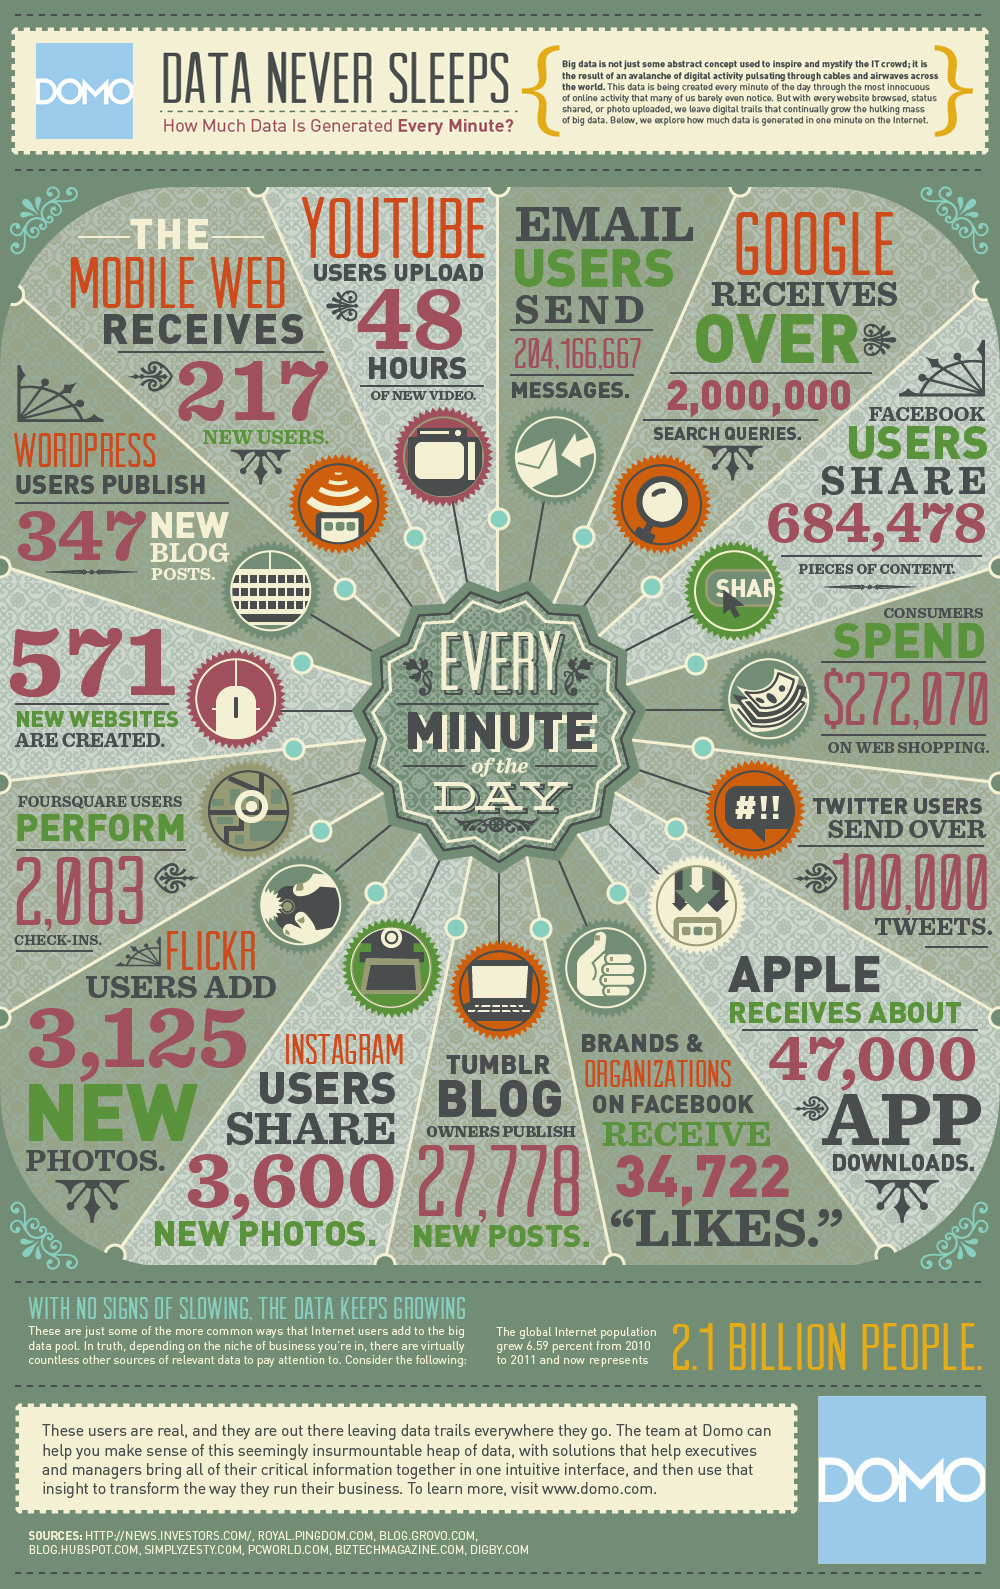
\includegraphics[width=0.48\textwidth]{Data-in-One-Minute.jpg}
	\caption{A simple caption}
	\label{data_per_minute}
\end{figure}
L'infografica nella figura \ref{data_per_minute}\footnote{\url{http://www.visualnews.com/2012/06/19/how-much-data-created-every-minute/?view=infographic}} ci permette di vedere con immediatezza di quali quantità stiamo parlando, e possiamo evincere che per una tale mole di informazioni occorrono delle procedure di trattamento dell'informazione diverse da quelle che possono essere adottate da un semplice programma per gestire una semplice rubrica. Stiamo parlando quindi di diversi GigaByte se non TeraByte di dati, che hanno bisogno di essere analizzati e processati in tempo modesto. I tipi di elaborazione necessari possono essere il calcolo di statistiche, una suddivisione per categoria, un'interrogazione della base di dati, oppure una serie di calcoli che possono permettere ad un'azienda di capire, in base agli acquisti dei suoi clienti, i trend riguardo alcuni suoi prodotti. Le tecniche elaborate nel corso degli anni hanno portato alla nascita di una nuova branca dell'informatica, quella dei \emph{Big Data}. Secondo \cite{rezzani2013big} una definizione di Big Data può essere:
\begin{quotation}
I BigData sono dati che superano i limiti degli strumenti di database tradizionali.
\end{quotation}
Con questo termine però non si intendono solo i dataset di grandi dimensioni, ma anche le tecniche utilizzate per elaborarli ed estrarre informazioni significative da esso.
Chiariamo l'\emph{obbiettivo} di questo processo, ossia la possibilità di poter elaborare delle informazioni significative 